%%%%%%%%%%%%%%%%%%%%%%%%%%%%%%%%%%%%%%PREAMBLE
\documentclass{article}


\usepackage{authblk}
\usepackage{Sweave}
\usepackage{graphicx}
\usepackage{tabularx}
\usepackage{hyperref}
\usepackage{natbib}
\usepackage{pdflscape}
\usepackage{array}
\usepackage{gensymb}
\usepackage{amsmath}
\usepackage{longtable}
\usepackage{xr}
\renewcommand{\baselinestretch}{1.8}
%\usepackage{lineno}
%\usepackage[backend=bibtex]{biblatex}
%Strongly recommended
 %put your figures in one place
 
%you'll want these for pretty captioning
\usepackage[small]{caption}

\setkeys{Gin}{width=0.8\textwidth} %make the figs 50 perc textwidth
\setlength{\captionmargin}{30pt}
\setlength{\abovecaptionskip}{0pt}
\setlength{\belowcaptionskip}{10pt}
% manual for caption http://www.dd.chalmers.se/latex/Docs/PDF/caption.pdf

%Optional: I like to muck with my margins and spacing in ways that LaTeX frowns on
%Here's how to do that
 \topmargin -2cm 
 \oddsidemargin -0.04cm 
 \evensidemargin -0.04cm % same as oddsidemargin but for left-hand pages
 \textwidth 16.59cm
 \textheight 22.94cm 
 %\pagestyle{empty} % Uncomment if don't want page numbers
 %\parskip 7.2pt  % sets spacing between paragraphs
 %\renewcommand{\baselinestretch}{1.5} 	% Uncomment for 1.5 spacing between lines
\parindent 0pt% sets leading space for paragraphs
\usepackage[doublespacing]{setspace}
%\doublespacing

%Optional: I like fancy headers
\usepackage{fancyhdr}
\pagestyle{fancy}
\fancyhead[LO]{Soil moisture and plant phenology}
\fancyhead[RO]{2018}

%%%%%%%%%%%%%%%%%%%%%%%%%%%%%%%%%%%%%%E

%Start of the document
\begin{document}

% \SweaveOpts{concordance=TRUE}
\bibliographystyle{amnat.bst}

\title{Supplemental Materials for \emph{Drier soils delay plant phenology across climate change experiments in temperate forest and grassland systems}}

%%%%%%%%%%%%%%%%%%%%%%%%%%%%%%%%%%%%%%%%%%%%%%%%%%%
%\linenumbers

\section* {Supplemental Methods}
\par The hierarchical linear phenology models we fit included response variable (\textit{y}), which represents day of year of the phenological event (budburst, leafout, or flowering). Predictors were measured air temperature (\textit{T}) and soil moisture(\textit{SM}), which were standardized by substracting the mean and divding by the standard deviation. Random effects are species (sp, random slopes and intercepts), and site and year nested within site (random intercepts only); $i$ represents each observation. 

\begin{align*}
\begin{equation}
y_{i}=\alpha_{sp[i],site[year[i]]} + \beta_{temp_{sp[i]}}+ \beta_{mois_{sp[i]}} + \beta_{temp:mois_{sp[i]}}+\epsilon_{i}\label{eq:8}
\end{equation}

\begin{equation}
\alpha_{sp}\sim N(\mu_{sp}, \sigma_{sp})
\end{equation}

\begin{equation}
\mu_{site[year]} \sim N(\mu_{siteyr}, \sigma_{siteyr})
\end{equation}

\begin{equation}
\mu_{site} \sim N(\mu_{site}, \sigma_{site})
\end{equation}

\begin{equation}
\beta_{temp_{sp}} \sim N(\mu_{\beta_{temp}}, \sigma_{\beta_{temp}})
\end{equation}

\begin{equation}
\beta_{mois_{sp}} \sim N(\mu_{\beta_{mois}}, \sigma_{\beta_{mois}})
\end{equation}

\begin{equation}
\beta_{temp:mois_{sp}} \sim N(\mu_{\beta_{temp:mois}}, \sigma_{\beta_{temp:mois}})
\end{equation}
\end{align*}

% \underline{Equations for soil moisture and temperature models}: 
% The equations below represent the models we used to understand effects of experimental temperature (\textit{eT}) and experimental preciptation (\textit{eP}) treatments treatments on soil moisture and temperature. Since the model structures for our analyses of moisture and temperature were identical, \textit{y} represents either moisture or temperature. 
% 
% \begin{equation}
% y_{i}=\alpha_{site[year[doy[i]]]}+ \beta_{temp_{site[i]}}eT_i+\beta_{2 site[i]}eP_i+\beta_{3 site[i]}eT_ieP_i+\epsilon_{i}\label{eq:1}
% \end{equation}
% \begin{equation}
% \alpha_{site[year[doy]]}\sim N(\mu_{site[year]}, \sigma_{site[year]})\label{eq:2}
% \end{equation}
% 
% \begin{equation}
% \mu_{site[year]} \sim N(\mu_{sy}, \sigma_{sy})\label{eq:3}
% \end{equation}
% 
% \begin{equation}
% \mu_{sy} \sim N(\mu_{s}, \sigma_{s})\label{eq:4}
% \end{equation}
% 
% \begin{equation}
% \beta_{1 site} \sim N(\mu_{\beta1}, \sigma_{\beta1})\label{eq:5}
% \end{equation}
% 
% \begin{equation}
% \beta_{2 site} \sim N(\mu_{\beta2}, \sigma_{\beta2})\label{eq:6}
% \end{equation}
% 
% \begin{equation}
% \beta_{3 site} \sim N(\mu_{\beta3}, \sigma_{\beta3})\label{eq:7}
% \end{equation}
% 
% 
% 
% \section* {Results}
% \begin{singlespace}


\bibliography{../../Bibliography/mylibrary.bib}

\section*{References to include}
\begin{itemize}
\item Later flowering is  associated with low precipitation, at least in part (Crimmins et al 2010)
\item Ganjurjav et al 2020
\item Cabon 2020
\end{itemize}

\clearpage
\section* {Supplemental Tables}

% latex table generated in R 4.4.1 by xtable 1.8-4 package
% Wed Oct 30 14:37:49 2024
\begin{table}[ht]
\centering
\caption{\textbf{Experimental sites and phenophases included in the ExPhen database}. Experimental sites correspond to the map (Figure S1). We give the study ID, location, source, years of data included, ecosystem, number of species, and phenophases included: budburst (bb), leafout (lo), flowering (fl), fruiting (fr), or senesence (sen) day of year. Note that some sites may have multiple sources; however, we list only one here. * denotes phenophases not included in this paper, because they were measured in fewer than three experiments.} 
\label{tab:studylocs}
\begingroup\footnotesize
\begin{tabular}{|p{0.04\textwidth}|p{0.18\textwidth}|p{0.2\textwidth}|p{0.08\textwidth}|p{0.1\textwidth}|p{0.07\textwidth}|p{0.09\textwidth}|}
  \hline
study & location & source & data years & ecosystem & species & phenophases \\ 
  \hline
exp01 & Waltham, MA, USA & Hoeppner and Dukes 2012 & 2009-2011 & grassland & 44 & bb,lo,fl \\ 
   \hline
exp02 & Montpelier, France & Morin et al. 2010 & 2004 & temperate deciduous forest & 5 & fl,fr* \\ 
   \hline
exp03 & Duke Forest, NC, USA & Clark et al. 2014 & 2009-2014 & temperate deciduous forest & 37 & bb,lo \\ 
   \hline
exp04 & Harvard Forest, MA, USA & Clark et al. 2014 & 2009-2012 & temperate deciduous forest & 29 & bb,lo \\ 
   \hline
exp07 & Harvard Forest, MA, USA & Pelini et al. 2011 & 2010-2015 & temperate deciduous forest & 8 & bb,lo,sen* \\ 
   \hline
exp09 & Stone Valley Forest, PA, USA & Rollinson and Kaye 2012 & 2009-2010 & temperate deciduous forest & 120 & lo,fl,fr*,sen* \\ 
   \hline
exp10 & Duke Forest, NC, USA & Marchin et al. 2015 & 2010-2013 & temperate deciduous forest & 11 & bb,fl \\ 
   \hline
exp12 & Kessler Farm Field Laboratory, OK, USA & Sherry et al. 2007 & 2003 & grassland & 12 & fl,fr* \\ 
   \hline
\end{tabular}
\endgroup
\end{table}%\end{footnotesize} 

\clearpage
% latex table generated in R 4.4.1 by xtable 1.8-4 package
% Wed Oct 30 14:38:21 2024
\begin{table}[ht]
\centering
\caption{\textbf{Summaries of budburst, leafout, and flowering models} with centered predictors.} 
\label{tab:mods}
\begingroup\footnotesize
\begin{tabular}{|p{0.1\textwidth}|p{0.05\textwidth}p{0.03\textwidth}p{0.05\textwidth}p{0.05\textwidth}p{0.05\textwidth}p{0.05\textwidth}|p{0.02\textwidth}p{0.02\textwidth}p{0.04\textwidth}|p{0.02\textwidth}p{0.02\textwidth}p{0.04\textwidth}|p{0.02\textwidth}p{0.02\textwidth}p{0.04\textwidth}|}
  \hline & \multicolumn{6}{c |}{Average Effects} &\multicolumn{3}{c |}{Species Effects} &\multicolumn{3}{c |}{Site Effects}&\multicolumn{3}{c |}{Site-Year Effects}\\
  \hline
 & mean & error & 25\% & 75\% & 5\% & 95\% & mean & error & Ngrp & mean & error & Ngrp & mean & error & Ngrp \\ 
  \hline
BB$\mu_{\alpha}$ & 97.20 & 5.10 & 94.00 & 100.40 & 88.60 & 105.20 & 16.00 & 2.40 & 41 & 7.3 & 5 & 5 & 9.3 & 2.4 & 13 \\ 
  BB$\mu_{temp}$ & -7.90 & 2.10 & -9.20 & -6.50 & -11.30 & -4.50 & 11.40 & 1.60 &  &  &  &  &  &  &  \\ 
  BB$\mu_{mois}$ & -1.70 & 0.60 & -2.10 & -1.30 & -2.80 & -0.70 & 2.70 & 0.60 &  &  &  &  &  &  &  \\ 
  BB$\mu_{temp:mois}$ & 0.50 & 0.50 & 0.20 & 0.80 & -0.40 & 1.30 & 1.70 & 0.70 &  &  &  &  &  &  &  \\ 
   \hline
LO$\mu_{\alpha}$ & 129.90 & 11.00 & 123.20 & 136.40 & 111.90 & 147.90 & 12.20 & 2.10 & 137 & 24.3 & 10.4 & 5 & 12.5 & 4 & 13 \\ 
  LO$\mu_{temp}$ & -10.30 & 1.40 & -11.30 & -9.40 & -12.70 & -7.90 & 10.30 & 1.30 &  &  &  &  &  &  &  \\ 
  LO$\mu_{mois}$ & -0.40 & 0.90 & -1.00 & 0.20 & -2.00 & 1.00 & 3.80 & 1.10 &  &  &  &  &  &  &  \\ 
  LO$\mu_{temp:mois}$ & 0.50 & 0.70 & 0.10 & 1.00 & -0.60 & 1.60 & 4.60 & 0.60 &  &  &  &  &  &  &  \\ 
   \hline
FL$\mu_{\alpha}$ & 167.00 & 9.00 & 161.80 & 172.00 & 153.00 & 180.70 & 48.20 & 3.50 & 124 & 11.6 & 10 & 5 & 8 & 4.6 & 8 \\ 
  FL$\mu_{temp}$ & -7.90 & 1.30 & -8.80 & -7.10 & -10.20 & -5.80 & 6.20 & 1.20 &  &  &  &  &  &  &  \\ 
  FL$\mu_{mois}$ & -1.30 & 0.90 & -1.90 & -0.70 & -2.80 & 0.20 & 3.80 & 1.10 &  &  &  &  &  &  &  \\ 
  FL$\mu_{temp:mois}$ & -1.10 & 0.70 & -1.60 & -0.60 & -2.30 & 0.10 & 2.70 & 0.90 &  &  &  &  &  &  &  \\ 
   \hline
\end{tabular}
\endgroup
\end{table}
%comparison of control plots vs all plots

\section*{Supplemental Figures}
% \clearpage
%  \begin{figure}[h]
% \centering
%  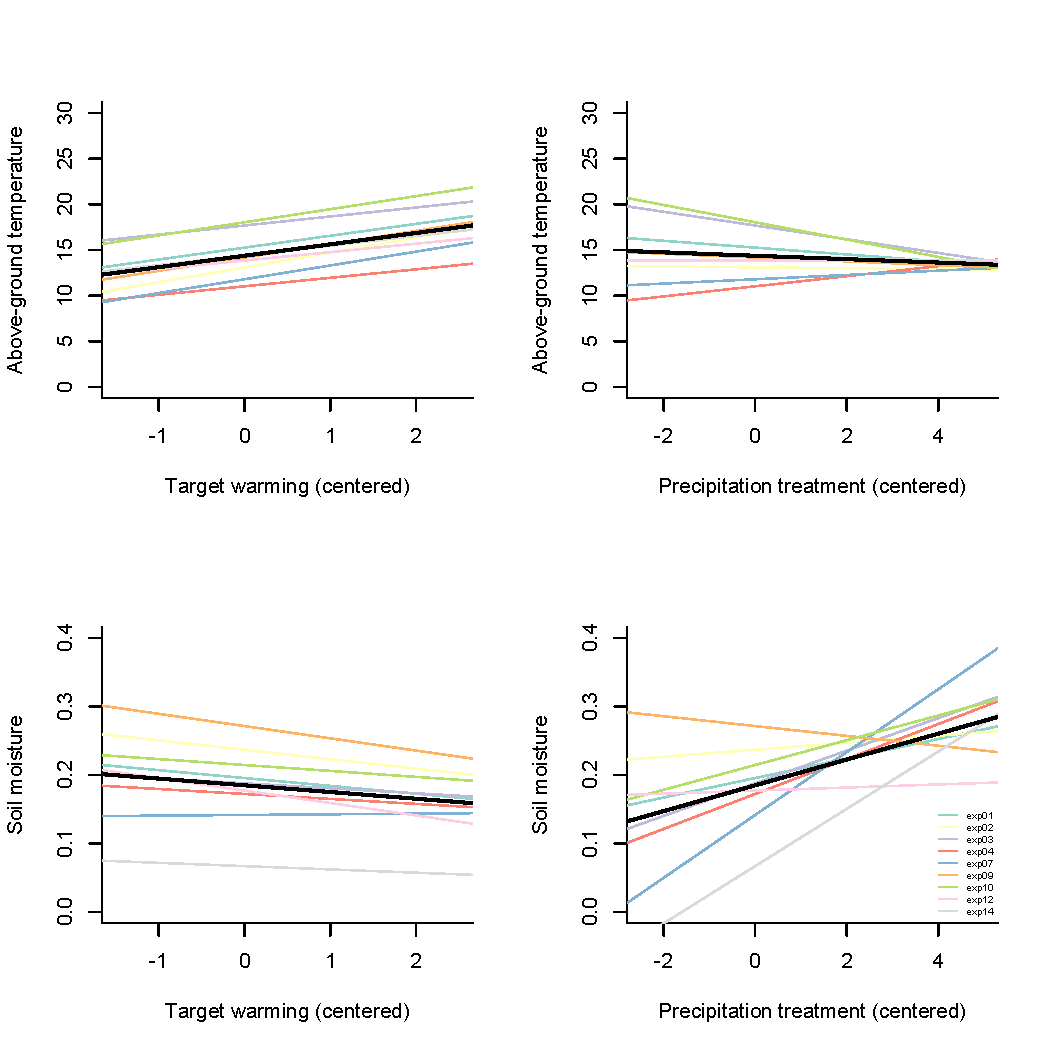
\includegraphics{../../Analyses/soilmoisture/figures/smtempvstargtemppreciptreat_lineslmerALL.pdf}
%  \caption{\textbf{Locations of experiments included in the meta-analysis.}} 
%  \label{fig:soilmois}
%  \end{figure}

% \clearpage
%  \begin{figure}[h]
% \centering
%  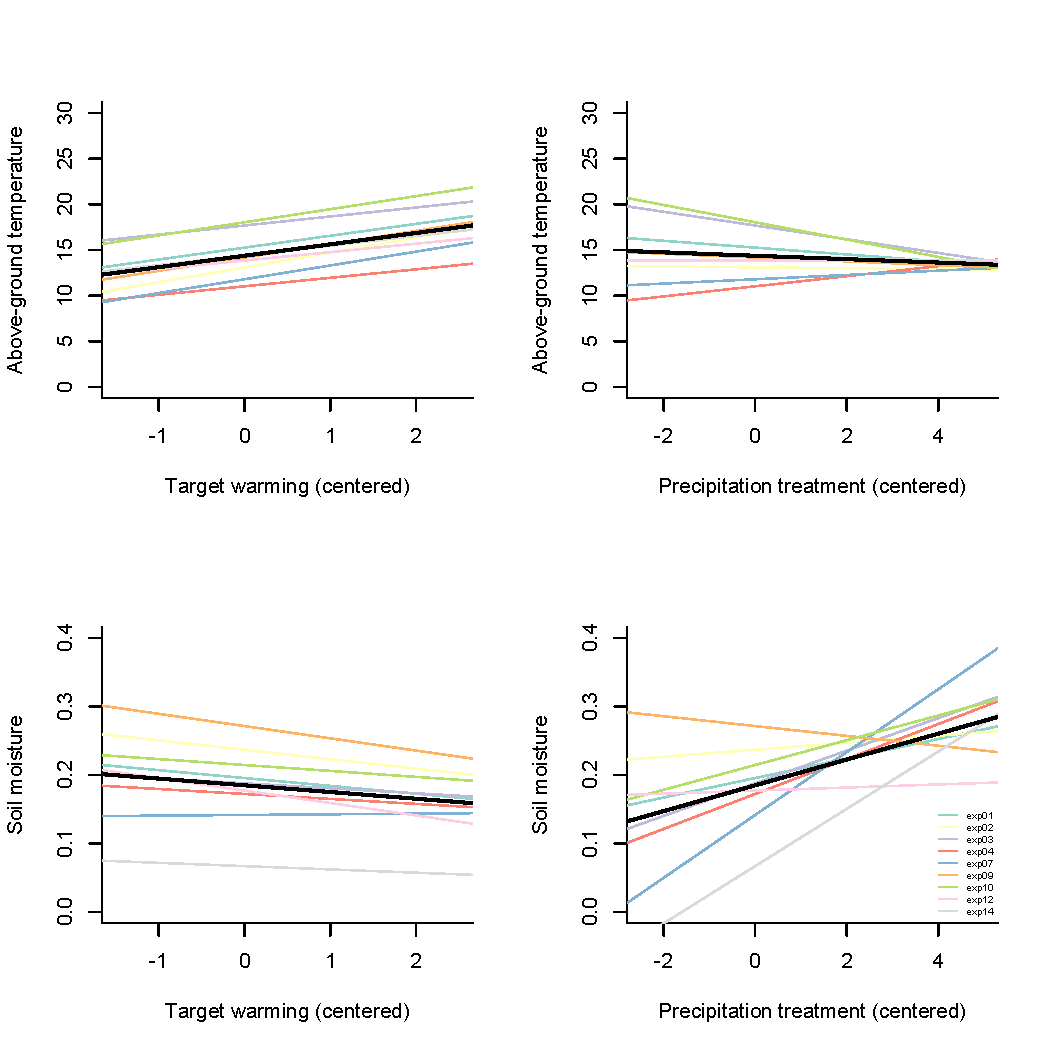
\includegraphics{../../Analyses/soilmoisture/figures/smtempvstargtemppreciptreat_lineslmerALL.pdf}
%  \caption{\textbf{Effects of target temperature and precipitation treatments on soil moisture.}} 
%  \label{fig:soilmois}
%  \end{figure}
% 

% \begin{figure}[h]
% \centering
%  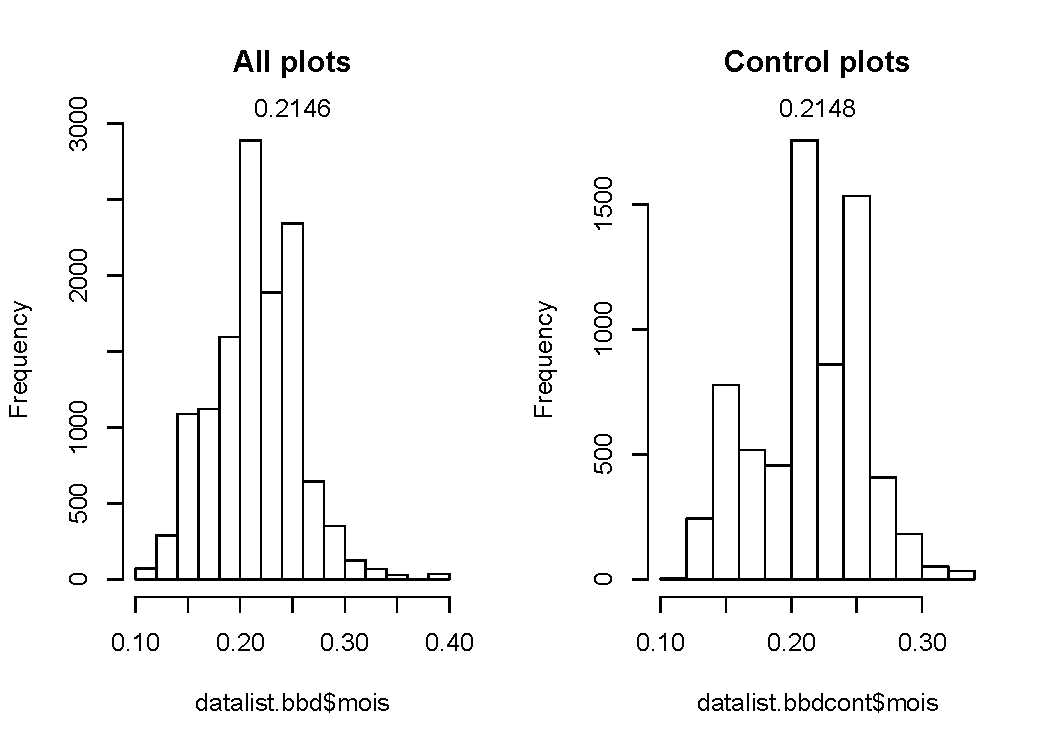
\includegraphics{../../Analyses/soilmoisture/figures/soilmoishist_mn.pdf}
%  \caption{\textbf{Observed daily soil moisture in all plots verus control plots.}} 
%  \label{fig:sm}
%  \end{figure}
% 
% \begin{figure}[h]
% \centering
%  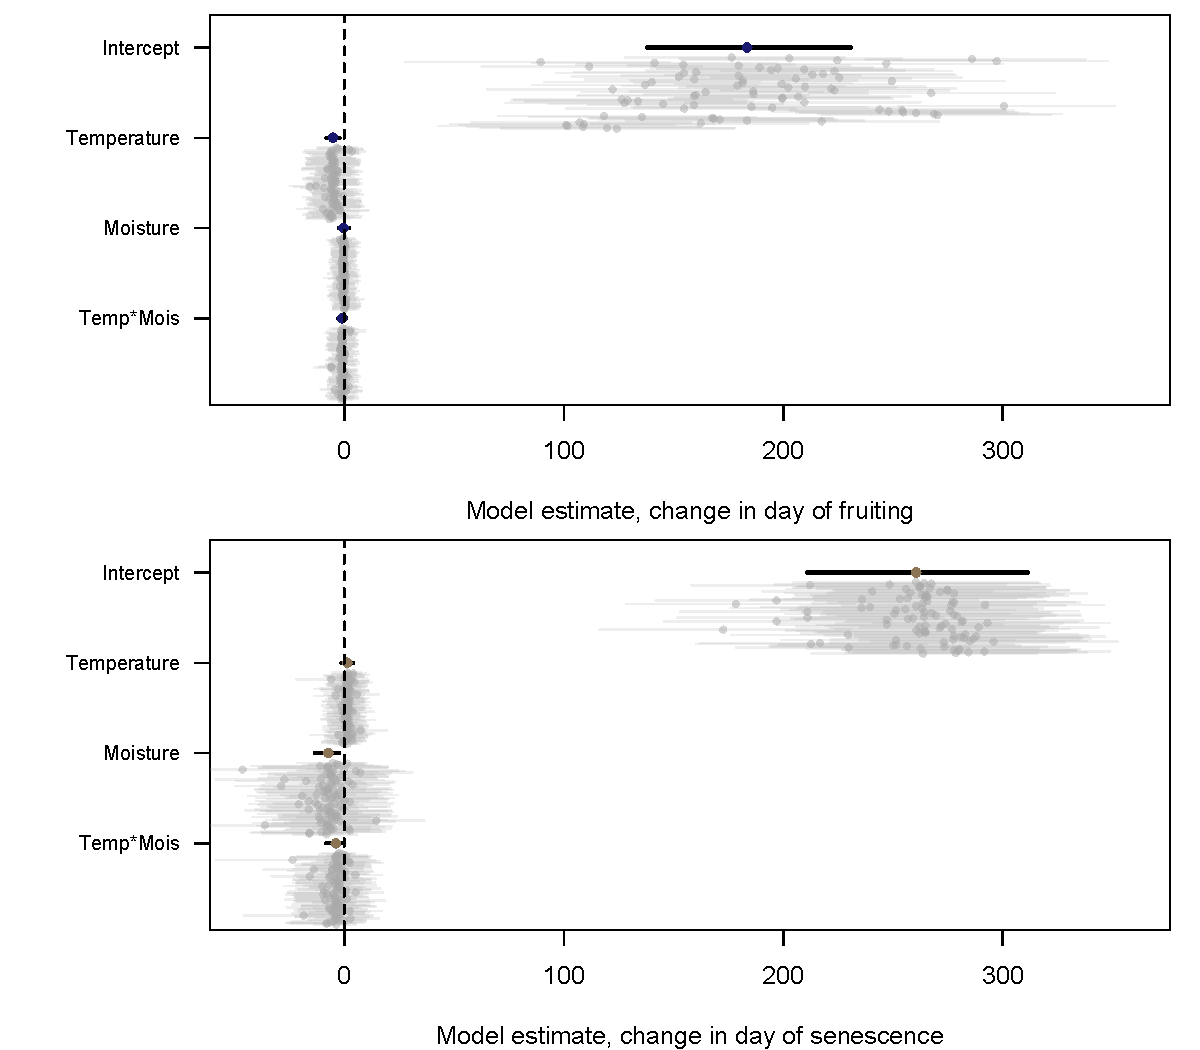
\includegraphics{../../Analyses/soilmoisture/figures/m5bffrdsen.pdf}
%  \caption{\textbf{Model coefficients from fruiting and senescence models (with centered predictors).}} 
%  \label{fig:ff}
%  \end{figure}
 \begin{figure}[h]
\centering
  \noindent\makebox[\textwidth]{%
 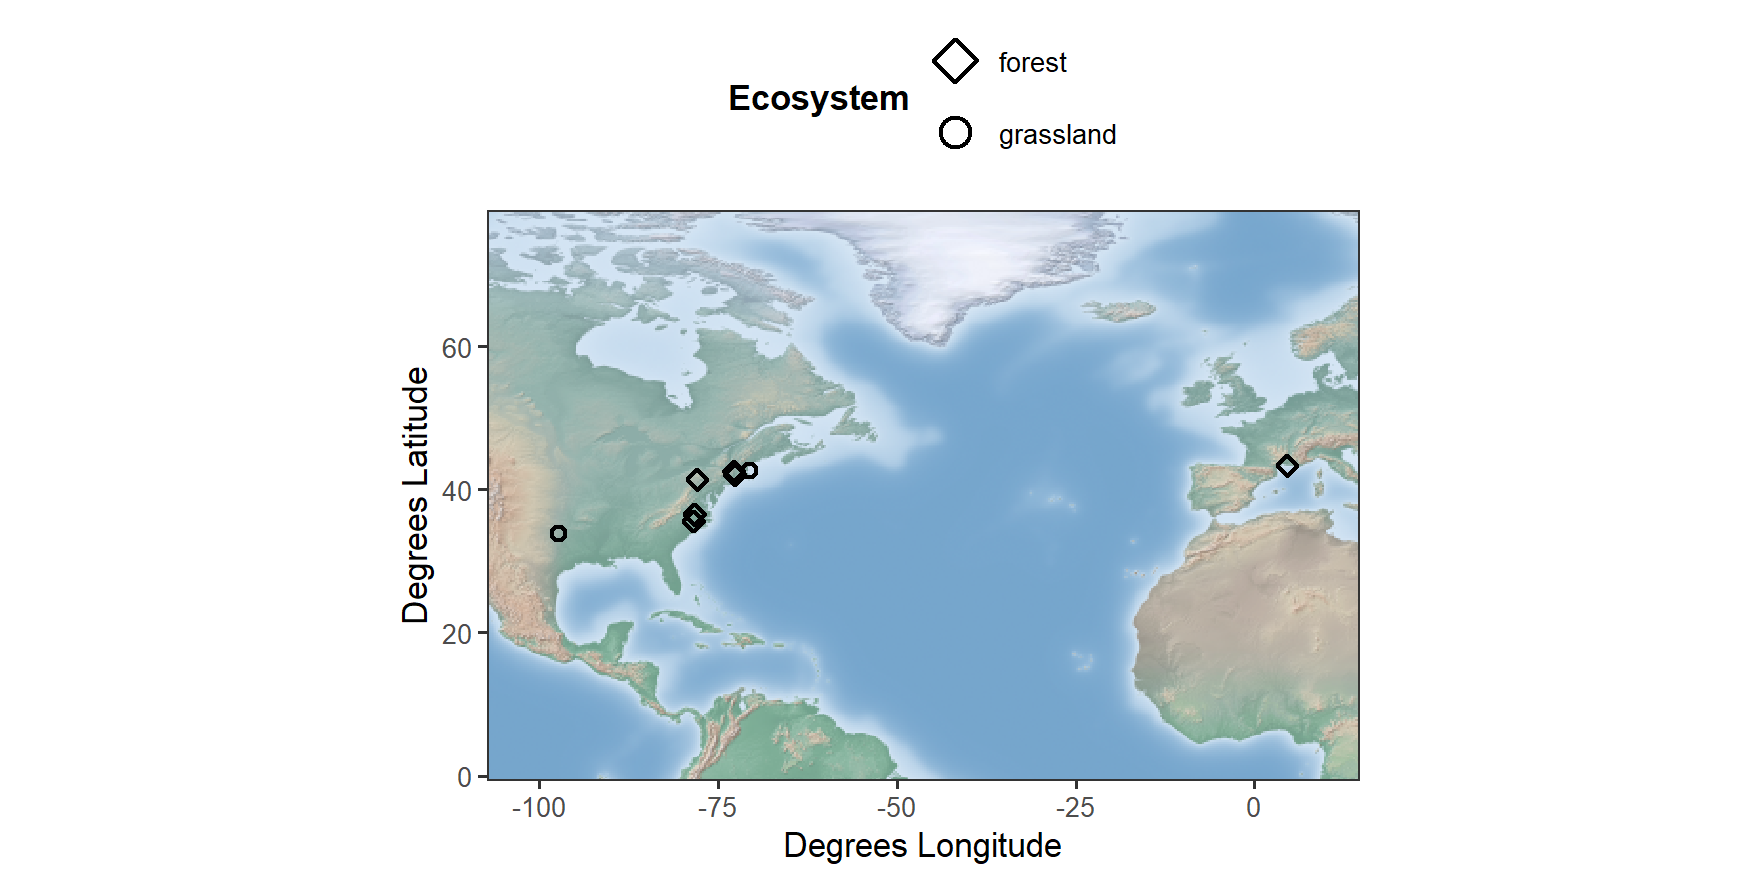
\includegraphics[width=1.5\textwidth]{../../Analyses/maps/soilms_experiments_map.png}}
 \caption{\textbf{Map of locations of experiments} included in this meta-analysis .Add phenophases to this, perhaps, by filling shapes with colors associated with phenophase} 
 \label{fig:map}
 \end{figure}

 \begin{figure}[h]
\centering
 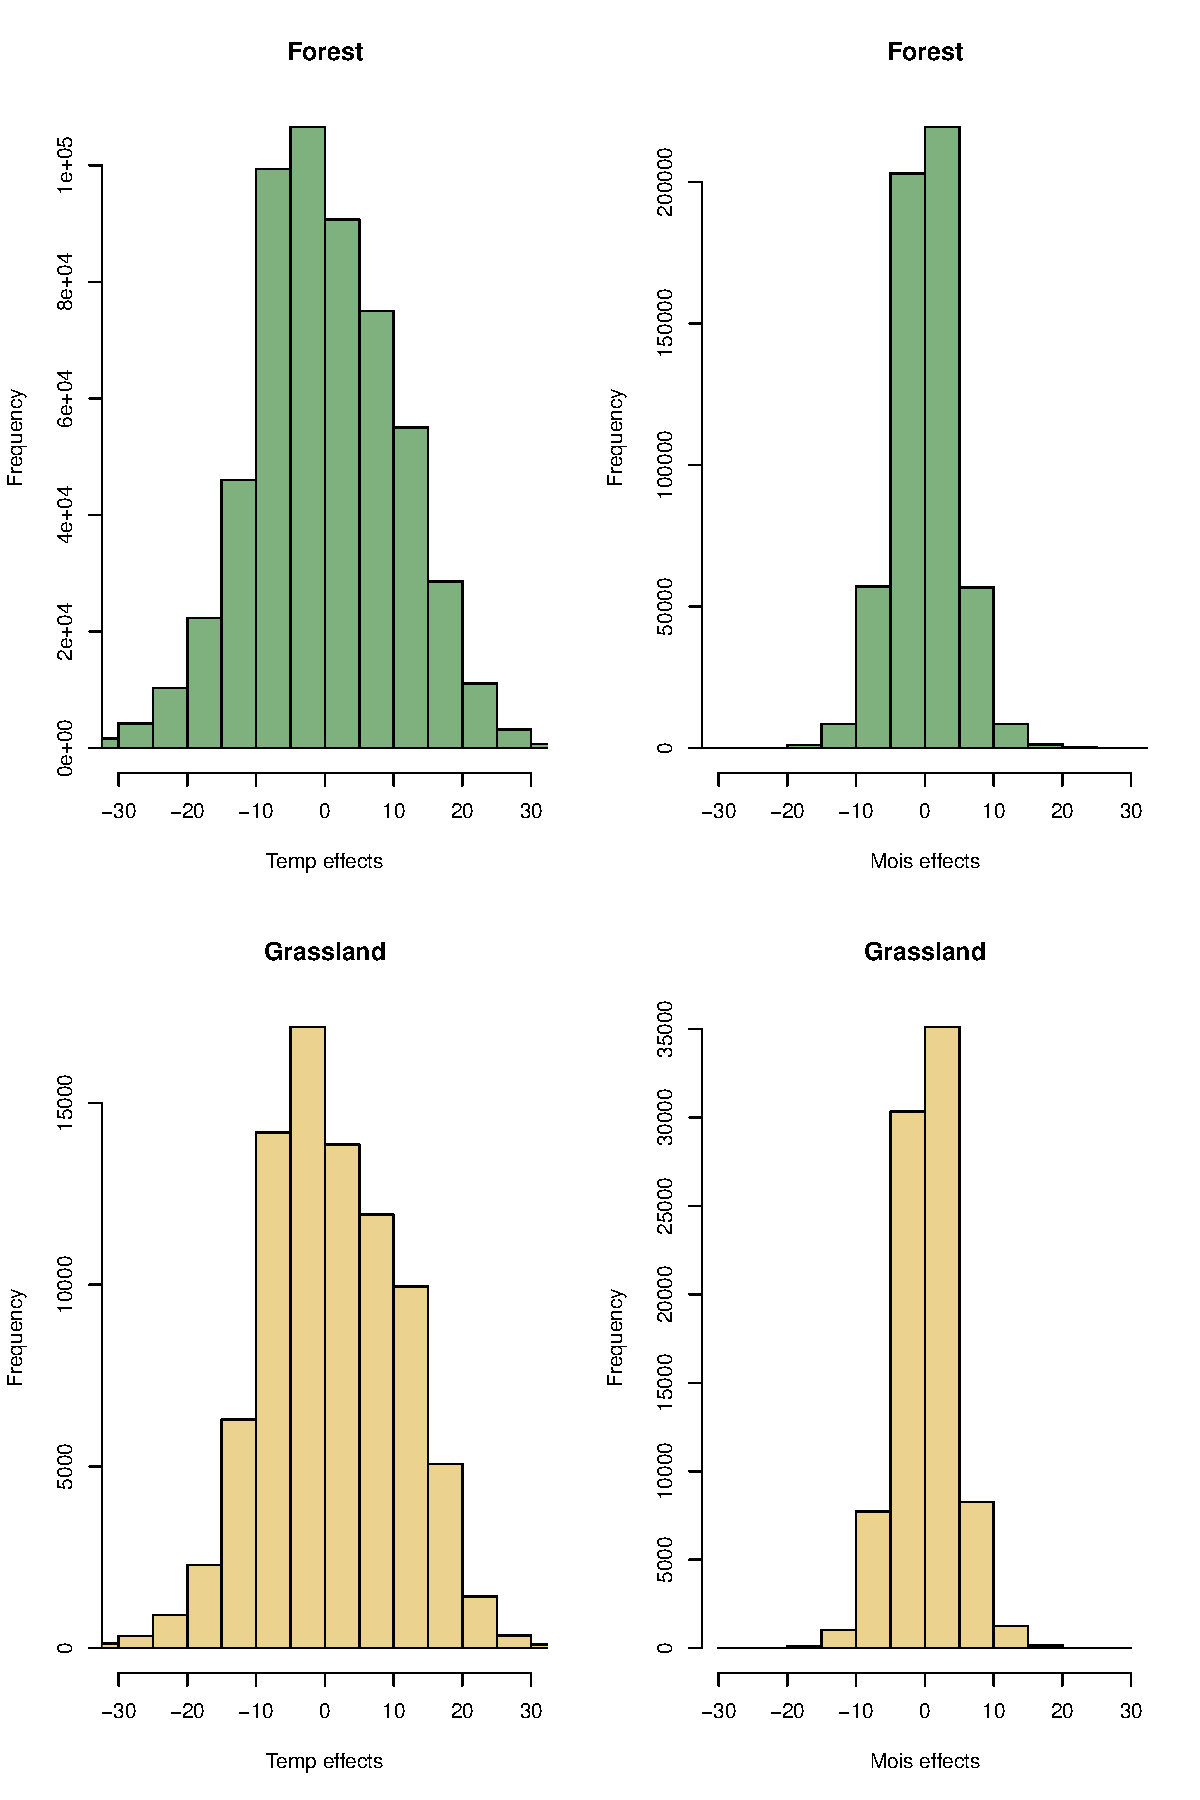
\includegraphics{../../Analyses/soilmoisture/figures/histloecos.pdf}
 \caption{\textbf{Effects of temperature and soil moisture do not differ strongly across ecosystems (forest vs grassland) for leafout (top) and budburst (bottom) models.}.}
 \label{fig:forms}
 \end{figure}
 
 Questions for co-authors:
 \begin{enumerate}
 \item Life forms vs ecosystems figures: Life forms plots histograms of speceis-level effects whereas ecosystems plots all posteriores (i.e. across 8000 samples)- what's your preference?
 \item Should I make plots of the distribution of soil moisture and temperature by site?

 \end{enumerate}
 
%%%%%%%%%%%%%%%%%%%%%%%%%%%%%%%%%%%%%%%%
\end{document}
%%%%%%%%%%%%%%%%%%%%%%%%%%%%%%%%%%%%%%%%
